\input{../YKY-preamble-PPT.tex}

\usepackage{color}
\usepackage{mathtools}
\usepackage{hyperref}

%\usepackage[backend=biber,style=numeric]{biblatex}
%\bibliography{../AGI-book}
% \renewcommand*{\bibfont}{\footnotesize}

\usepackage{graphicx} % Allows including images
\usepackage{tikz-cd}
\usepackage{tikz}
\usepackage[export]{adjustbox}% http://ctan.org/pkg/adjustbox
\usepackage{verbatim} % for comments
% \usepackage{newtxtext,newtxmath}	% Times New Roman font

% \numberwithin{equation}{subsection}

\newcommand{\underdash}[1]{%
	\tikz[baseline=(toUnderline.base)]{
		\node[inner sep=1pt,outer sep=10pt] (toUnderline) {#1};
		\draw[dashed] ([yshift=-0pt]toUnderline.south west) -- ([yshift=-0pt]toUnderline.south east);
	}%
}%

\DeclareSymbolFont{symbolsC}{U}{txsyc}{m}{n}
\DeclareMathSymbol{\strictif}{\mathrel}{symbolsC}{74}

\newcommand{\highlight}[1]{\colorbox{pink}{$\displaystyle #1$}}

\newcommand{\emp}[1]{{\color{blue}\textbf{#1}}}
\newcommand*\confoundFace{$\vcenter{\hbox{\includegraphics[scale=0.2]{../2020/../confounded-face.jpg}}}$}
\newcommand{\underconst}{\includegraphics[scale=0.5]{../2020/UnderConst.png}}
\newcommand{\witness}{\scalebox{0.6}{$\blacksquare$}}
% \newcommand{\Heytingarrow}{\mathrel{-}\mathrel{\triangleright}}
\providecommand\Heytingarrow{\relbar\joinrel\mathrel{\vcenter{\hbox{\scalebox{0.75}{$\rhd$}}}}}

\begin{document}

\title{\bfseries\color{blue}{\Huge《AGI in 5 minutes》}}
\author{YKY} % Your name
%\institute[] % Your institution as it will appear on the bottom of every slide, may be shorthand to save spacer5t
%{
%Independent researcher, Hong Kong \\ % Your institution for the title page
%\medskip
%\textit{generic.intelligence@gmail.com} % Your email address
%}
\date{\today} % Date, can be changed to a custom date

\maketitle
\pagenumbering{gobble}

\begin{itemize}
	\item 我预计 AGI 会在 5-6 年内出现。
	\item 理由是 因为 BERT/GPT 已经示范了 \\
		 现时计算机的算力 \\
		 已经进入了 AGI 的 ``ballpark'' 范围
	\item BERT/GPT 可以 答问题、写文章、甚至写 code,\\
		这些能力 毫无疑问是 通用智能 的特性
	\item 虽然很多人见到了 BERT/GPT,\\
		但并不意识到它们就是 AGI 的雏型
\end{itemize}

\section{1st-gen AGI}



\begin{equation}
\vcenter{\hbox{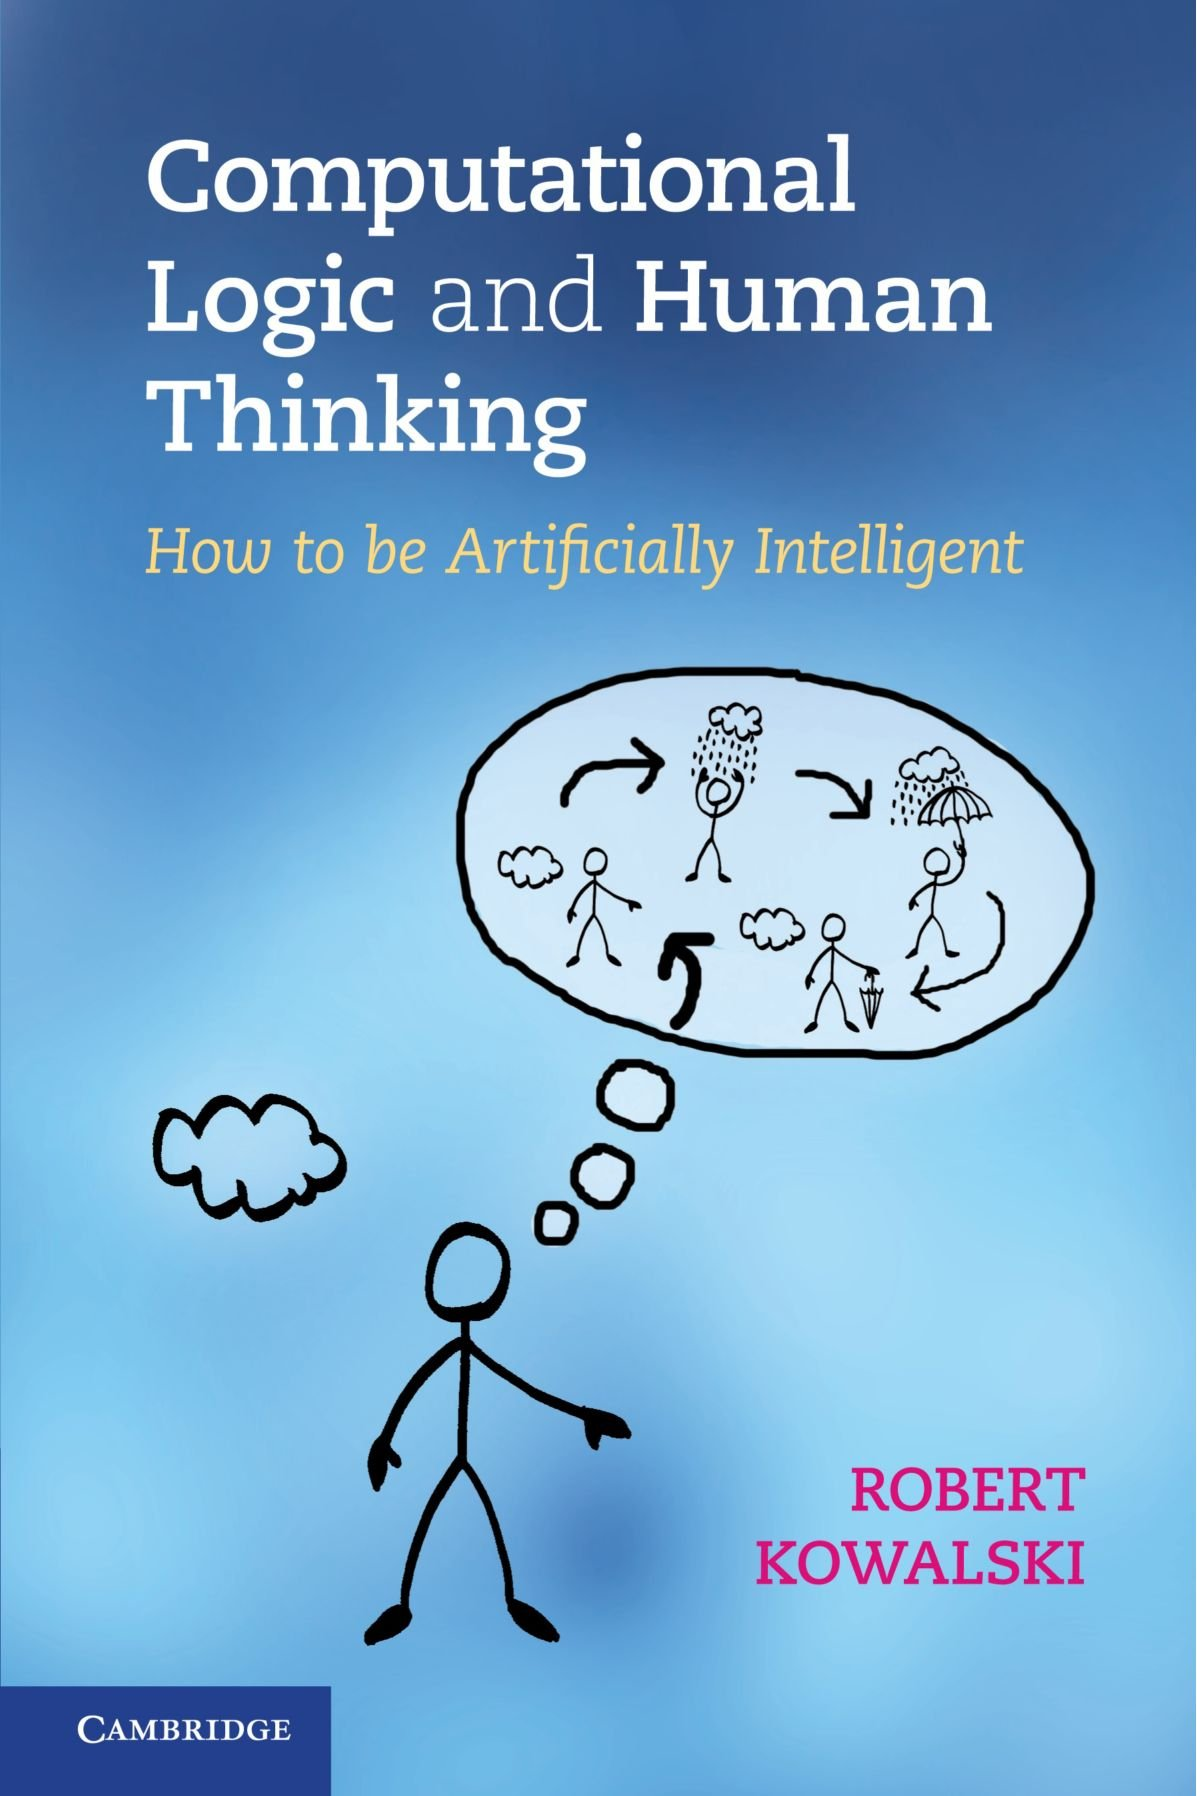
\includegraphics[scale=0.3]{Computational-logic-and-human-thinking_(cover).jpg}}}
\end{equation}

\begin{equation}
\vcenter{\hbox{
\includegraphics[scale=0.7]{Jerry-Hobbs.png}}}
\end{equation}

Novamente, Deep Mind

% \section*{References}
% \cc{欢迎提问和讨论}{Questions, comments welcome} \smiley \\ \vspace*{0.4cm}
% \printbibliography

\end{document}
